

%
\documentclass[10pt,journal,compsoc]{IEEEtran}
\usepackage[brazil]{babel}
\usepackage[utf8]{inputenc}		%Usar acentos diretos do teclado
\usepackage[T1]{fontenc}		%Padrão para imagens
\usepackage{graphicx}
\usepackage{subfigure}
\usepackage{rotating}
\usepackage{longtable}
\usepackage{amsmath}
\usepackage{amsfonts}
\usepackage{amssymb}
\usepackage{geometry}
\usepackage{caption}
\ifCLASSOPTIONcompsoc
  % The IEEE Computer Society needs nocompress option
  % requires cite.sty v4.0 or later (November 2003)
  \usepackage[nocompress]{cite}
\else
  % normal IEEE
  \usepackage{cite}
\fi
\ifCLASSINFOpdf
 
\else

\fi




\newcommand\MYhyperrefoptions{bookmarks=true,bookmarksnumbered=true,
pdfpagemode={UseOutlines},plainpages=false,pdfpagelabels=true,
colorlinks=true,linkcolor={black},citecolor={black},urlcolor={black},
pdftitle={Bare Demo of IEEEtran.cls for Computer Society Journals},%<!CHANGE!
pdfsubject={Typesetting},%<!CHANGE!
pdfauthor={Michael D. Shell},%<!CHANGE!
pdfkeywords={Computer Society, IEEEtran, journal, LaTeX, paper,
             template}}%<^!CHANGE!
%\ifCLASSINFOpdf
\hyphenation{op-tical net-works semi-conduc-tor}


\begin{document}
%
\title{Estudo de Caso de um Problema do Autovalor Quadrático em um Modelo de Asa}
%
%

\author{Pedro~Gushiken,~\IEEEmembership{Member,~IEEE,}
        Isaac~Dantas,~\IEEEmembership{Member,~IEEE,}
\IEEEcompsocitemizethanks{\IEEEcompsocthanksitem P. Gushiken e I. Dantas estão no Programa de Pós-Graduação em Engenharia Elétrica e da Computação como mestrandos, Universidade Federal do Rio Grande do Norte , Natal, Laboratório de Automação, Controle e Instrumentação .\protect\\
% note need leading \protect in front of \\ to get a newline within \thanks as
% \\ is fragile and will error, could use \hfil\break instead.
E-mail: pedrogush@gmail.com
}% <-this % stops a space
\thanks{Manuscrito recebido dia 15 de dezembro, 2016}}

% The paper headers
\markboth{Coleção, Trabalhos NLEVP}%
{Shell \MakeLowercase{\textit{et al.}}: Bare Advanced Demo of IEEEtran.cls for IEEE Computer Society Journals}

\IEEEtitleabstractindextext{%
\begin{abstract}
We studied the behavior of the eigenvalues of the 'wing' problem presented in the NLEVP collection of quadratic eigenvalue problems(QEPs) for each matrix $A_2$, $A_1$ and $A_0$ as a way of understanding possible applications of QEPs in real world settings. The eigenvalues represent the behavior of the oscillations of the wing.
\end{abstract}

% Note that keywords are not normally used for peerreview papers.
\begin{IEEEkeywords}
NLEVP, QEP, wing
\end{IEEEkeywords}}


% make the title area
\maketitle


\IEEEdisplaynontitleabstractindextext

\IEEEpeerreviewmaketitle


\ifCLASSOPTIONcompsoc
\IEEEraisesectionheading{\section{Introduction}\label{sec:introduction}}
\else
\section{Introduction}
\label{sec:introduction}
\fi
\IEEEPARstart{O} problema do autovalor quadrático tem uma série de aplicações. Nos foi pedido a escolha de um dos 54 problemas contidos no toolbox NLEVP(citar manual). Escolhemos o problema wing(citar artigos) e simulamos a posição dos autovalores variando individualmente cada matriz.  
% You must have at least 2 lines in the paragraph with the drop letter
% (should never be an issue)

\subsection{Asa}
O problema escolhido se trata da modelagem das oscilações de uma asa de acordo com matrizes de $M,C,K$, de Massa, Atrito e Amortecimento respectivamente. Esperamos que a medida que a matriz de massa $M$ tenha sua norma reduzida as oscilações se tornem mais amortecidas, isto é, autovalores mais à esquerda no semi plano esquerdo. Enquanto que para as matrizes de atrito e amortecimento $C,K$ as oscilações se tornem cada vez menos amortecidas até que se tornem instáveis, o que seria caracterizado por autovalores do feixe localizados no semiplano direito aberto.

% needed in second column of first page if using \IEEEpubid
%\IEEEpubidadjcol

\section{Caracterização}
Este problema de um polinômio matricial $3\times3$ quadrático surge a partir do estudo de (Frazer, citar), modificado numericamente como em (Lancaster, citar) e é da forma:

\[
Q(\lambda) = \lambda^2A_2 + \lambda A_1 + A_0
\]

O problema surge a partir da análise de um modelo de asa submetido a um fluxo de ar. As matrizes são:

\[
A_2 = \begin{bmatrix}
17.6 & 1.28 & 2.89\\
1.28 & 0.824 & 0.413\\
2.89 & 0.413 & 0.725
\end{bmatrix}
,~~
A_1 = \begin{bmatrix}
7.66 & 2.45 & 2.1 \\
0.23 & 1.04 & 0.223\\
0.6 & 0.756 & 0.658
\end{bmatrix}
\]

\[
A_0 = \begin{bmatrix}
121 & 18.9 & 15.9\\
0 & 2.7 & 0.145 \\
11.9 & 3.64 & 15.5
\end{bmatrix}
\]

Em nosso estudo de caso escolhemos diminuir a norma de cada matriz individualmente, plotando o comportamento dos autovalores para cada caso. Para isso foi usado o script fornecido pelo professor José Mário, com algumas modificações:

\begin{verbatim}

clear all
close all
v = 0:0.01:1;
coeffs = nlevp('wing');
M = coeffs{1,3};
    C = coeffs{1,2};
    K = coeffs{1,1};
figure
hold
flagb = 0;
for l = 1:60
    M = M*0.95;
    lambda = polyeig(K,C,M);
    r_eig = real(lambda);
    i_eig = imag(lambda);
    plot(r-eig,i_eig,'.');
end
\end{verbatim}

E para a matriz C:
\begin{verbatim}

clear all
close all
v = 0:0.01:1;
coeffs = nlevp('wing');
M = coeffs{1,3};
    C = coeffs{1,2};
    K = coeffs{1,1};
figure
hold
flagb = 0;
for l = 1:60
    C = C*0.95;
    lambda = polyeig(K,C,M);
    r_eig = real(lambda);
    i_eig = imag(lambda);
    plot(r-eig,i_eig,'.');
end
\end{verbatim}


E para K:
\begin{verbatim}

clear all
close all
v = 0:0.01:1;
coeffs = nlevp('wing');
M = coeffs{1,3};
    C = coeffs{1,2};
    K = coeffs{1,1};
figure
hold
flagb = 0;
for l = 1:60
    K = K*0.95;
    lambda = polyeig(K,C,M);
    r_eig = real(lambda);
    i_eig = imag(lambda);
    plot(r-eig,i_eig,'.');
end
    
\end{verbatim}

\section{Resultados}

\begin{figure}[htpb!]
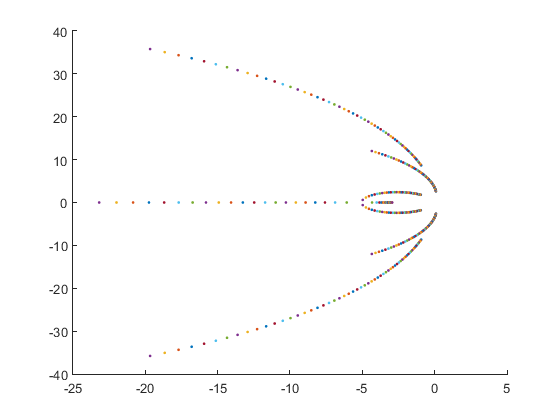
\includegraphics[width = \linewidth]{./pics/M.png}
\caption{Comportamento dos autovalores a medida que a norma de $A_2$ diminui}
\end{figure}

\begin{figure}[htpb!]
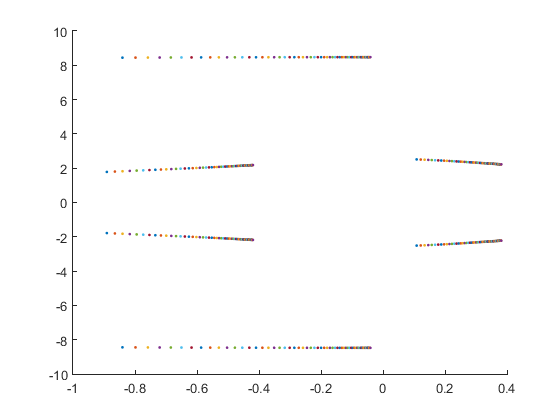
\includegraphics[width = \linewidth]{./pics/C.png}
\caption{Comportamento dos autovalores a medida que a norma de $A_1$ diminui}
\end{figure}

\begin{figure}[htpb!]
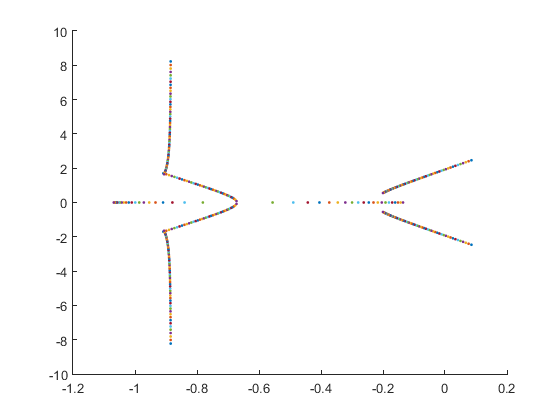
\includegraphics[width = \linewidth]{./pics/K.png}
\caption{Comportamento dos autovalores a medida que a norma de $A_0$ diminui}
\end{figure}
\pagebreak
\section{Conclusão}
Foi possível aplicar os conceitos relacionados ao problema do autovalor quadrático num caso já estudado na literatura. Fazendo uso do software MATLAB para a resolução do problema podemos fazer avaliações sobre a estabilidade do comportamento da asa submetida a um fluxo de ar.



% trigger a \newpage just 
\begin{thebibliography}{1}

\bibitem{IEEEhowto:kopka}
H.~Kopka and P.~W. Daly, \emph{A Guide to {\LaTeX}}, 3rd~ed.\hskip 1em plus
  0.5em minus 0.4em\relax Harlow, England: Addison-Wesley, 1999.

\end{thebibliography}

% biography section
% 
% If you have an EPS/PDF photo (graphicx package needed) extra braces are
% needed around the contents of the optional argument to biography to prevent
% the LaTeX parser from getting confused when it sees the complicated
% \includegraphics command within an optional argument. (You could create
% your own custom macro containing the \includegraphics command to make things
% simpler here.)
%\begin{IEEEbiography}[{\includegraphics[width=1in,height=1.25in,clip,keepaspectratio]{mshell}}]{Michael Shell}
% or if you just want to reserve a space for a photo:

% if you will not have a photo at all:

% insert where needed to balance the two columns on the last page with
% biographies
%\newpage


% You can push biographies down or up by placing
% a \vfill before or after them. The appropriate
% use of \vfill depends on what kind of text is
% on the last page and whether or not the columns
% are being equalized.

%\vfill

% Can be used to pull up biographies so that the bottom of the last one
% is flush with the other column.
%\enlargethispage{-5in}



% that's all folks
\end{document}


